\documentclass[12pt]{report}
\usepackage{setspace}  %use this package to set linespacing as desired
\usepackage{array}
\usepackage{graphicx}
\usepackage{subcaption}
\usepackage{amsmath}
\usepackage[counterclockwise, figuresleft]{rotating}

\begin{document}
\doublespacing

\clearpage
\chapter{Results}

\section{Correlation of Parameters} \label{section:corrofparams}

We observe correlation between two parameters using the statistical definition of the correlation coefficient ($\rho_{X,Y}$), defined as

\begin{equation}
\rho_{X,Y} = \dfrac{cov(X,Y)}{\sigma_X\sigma_Y}
\end{equation}

where \textit{cov} represents covariance. The correlation coefficient is unit-less, and measured from -1.0 $<$ $\rho_{X,Y}$ $<$ 1.0. A correlation coefficient of 0 indicates the variables X and Y are uncorrelated, while -1.0 indicates the variables are perfectly inversely correlated; likewise, a correlation coefficient of 1.0 means X and Y are perfectly correlated. Correlation coefficient is used to estimate an environmental parameter's potential usefulness for calculating a new \textit{coneR1} for use in an arbitrary environment.

\subsection{\textit{coneR1} and Average Attenuation} \label{section:coner1andatten}

Both attenuation models (dB and \%$\Delta$) were considered for correlation against optimal \textit{coneR1} values. Results for both are visualized below (Figure \ref{fig:corr_db} and Figure \ref{fig:corr_rgb}). Visualization demonstrates that while correlation coefficient describes the relationship of the two sets (optimal \textit{coneR1} and attenuation) at a superficial level, it cannot describe any translation that may be needed between the two sets.

% dB correlation
\begin{figure}
  \centering
  \begin{subfigure}{1\linewidth}
  \includegraphics[width=1\linewidth]{figures/correlations/db/room_hsv.jpg}
  \caption{}
\end{subfigure}
\hfill
\begin{subfigure}{.49\linewidth}
  \includegraphics[width=1\linewidth]{figures/correlations/db/campus_hsv.jpg}
  \caption{}
\end{subfigure}
\begin{subfigure}{.49\linewidth}
  \includegraphics[width=1\linewidth]{figures/correlations/db/pets2_hsv.jpg}
  \caption{}
\end{subfigure}

\caption{Visualization of the correlation discovered between the average attenuation (dB model) of dark shadow pixels, and the \textit{coneR1} algorithmic parameter. All results can be found in the appendix.}
\label{fig:corr_db}
\end{figure}

Tables \ref{table:corr_db} and \ref{table:corr_rgb} present correlation coefficients for each dataset for the dB model and \%$\Delta$ models of attenuation. The variance of both sets of correlated data is included as additional information, to better illustrate the relationship between the sets. For example, while sets of similar variance trend towards higher correlation coefficients, a dataset such as aton\_highway3 may have a high correlative factor despite dissimilar variances. Such anomalies indicate that non-correlative data points within a set are due to uncharacteristic spikes in either dataset, rather than a general trend of disassociation.

% Table Form (dB)
\begin{table}
\centering
\begin{tabular}{ |c|c|c|c| }
	\hline
	\textbf{Dataset} & \textbf{$\sigma_{coneR1}$} & \textbf{$\sigma_{dB}$} & \textbf{$\rho$} \\
	\hline
	\hline
	\textbf{PETS1} & 0.00076 & 0.00780 & 0.19855 \\
	\hline
	\textbf{PETS2} & 0.01221 & 0.01167 & 0.67058 \\
	\hline
	\textbf{aton\_highway1} & 0.00087 & 0.00020 & 0.68368 \\
	\hline
	\textbf{aton\_highway3} & 0.03031 & 0.00283 & 0.74241 \\
	\hline
	\textbf{aton\_room} & 0.00523 & 0.01957 &  0.54775 \\
	\hline
	\textbf{aton\_campus} & 0.00761 & 0.00270 &  0.35996 \\
	\hline
	\textbf{aton\_hallway} & 0.00664 & 0.00439 &  0.65615 \\
	\hline
	\textbf{aton\_lab} & 0.00902 & 0.01697 &  0.69540 \\
	\hline
\end{tabular}
\caption{Datasets and their correlations to \textit{coneR1} (dB model).}
\label{table:corr_db}
\end{table}

% RGB model
\begin{figure}
  \centering
  \begin{subfigure}{1\linewidth}
  \includegraphics[width=1\linewidth]{figures/correlations/rgb/room_hsv.jpg}
  \caption{}
\end{subfigure}
\hfill
\begin{subfigure}{.49\linewidth}
  \includegraphics[width=1\linewidth]{figures/correlations/rgb/campus_hsv.jpg}
  \caption{}
\end{subfigure}
\begin{subfigure}{.49\linewidth}
  \includegraphics[width=1\linewidth]{figures/correlations/rgb/pets2_hsv.jpg}
  \caption{}
\end{subfigure}

\caption{Visualization of the correlation discovered between the average attenuation (\%$\Delta$ model) of dark shadow pixels, and the \textit{coneR1} algorithmic parameter. All results can be found in the appendix.}
\label{fig:corr_rgb}
\end{figure}

% Table Form (RGB)
\begin{table}
\centering
\begin{tabular}{ |c|c|c|c| }
	\hline
	\textbf{Dataset} & \textbf{$\sigma_{coneR1}$} & \textbf{$\sigma_{\%\Delta}$} & \textbf{$\rho$} \\
	\hline
	\hline
	\textbf{PETS1} & 0.00076 & 0.00904 & 0.18377 \\
	\hline
	\textbf{PETS2} & 0.01221 & 0.01078 & 0.74308 \\
	\hline
	\textbf{aton\_highway1} & 0.00086 & 0.00010 & 0.59231 \\
	\hline
	\textbf{aton\_highway3} & 0.03030 & 0.00571 &  0.80138 \\
	\hline
	\textbf{aton\_room} & 0.00522 & 0.01890 &  0.62269 \\
	\hline
	\textbf{aton\_campus} & 0.00761 & 0.00323 &  0.56459 \\
	\hline
	\textbf{aton\_hallway} & 0.00664 & 0.00416 &  0.68973 \\
	\hline
	\textbf{aton\_lab} & 0.00902 & 0.01164 &  0.55087 \\
	\hline
\end{tabular}
\caption{Datasets and their correlations to \textit{coneR1} (\%$\Delta$ attenuation model).}
\label{table:corr_rgb}
\end{table}

PETS1 serves as the primary outlier with a correlation coefficient of approximately 19\% for both attenuation models. One of the primary culprits is the lack of a properly adaptive background model for the dataset, i.e., a frame may contain extreme cloud cover, while its corresponding background model retains its sunny disposition. The resultant of the non-ideal background model is that every pixel contained in the foreground has a greater attenuation when compared to its background pixel, excluding natural cast shadows, whose attenuation remains relatively consistent. This large swing in overall attenuation impacts the amount of pixels considered for candidacy by Physical removal's weak detector. The discrepancy found in the correlation coefficient of PETS1 is the result of the flood of non-shadow candidate pixels. While both PETS2 and PETS1 experience illumination change within the extracted samples, PETS2 does not endure the same measure of disrelation. The illumination change in PETS2 causes less intensity differential, allowing for shadow pixels to remain distinct. 

Both the dB and \%$\Delta$ attenuation models are visualized to contrast the trends of each method of calculation. Direct qualitative comparison is found in Figure \ref{fig:corr_compare}. 

The results in Tables \ref{table:corr_db} and \ref{table:corr_rgb} indicate that some datasets benefit from the dB attenuation model, while others benefit from the \%$\Delta$ attenuation model. Due to the multiplicative nature of the dB calculation, some data points are exaggerated, causing correlation increase within some environments, and decrease in others. While the correlation found using the dB and \%$\Delta$ models are comparable, the \%$\Delta$ attenuation model is used in the general model for improvement proposed. This is due to the \%$\Delta$ model requiring less translation from calculated attenuation to optimal \textit{coneR1}.

% Compare RGB to dB
\begin{figure}
\centering
\begin{subfigure}{.49\linewidth}
  \includegraphics[width=1\linewidth]{figures/correlations/db/room_hsv.jpg}
  \caption{}
\end{subfigure}
\hfill
\begin{subfigure}{.49\linewidth}
  \includegraphics[width=1\linewidth]{figures/correlations/rgb/room_hsv.jpg}
  \caption{}
\end{subfigure}
\hfill
\begin{subfigure}{.49\linewidth}
  \includegraphics[width=1\linewidth]{figures/correlations/db/campus_hsv.jpg}
  \caption{}
\end{subfigure}
\begin{subfigure}{.49\linewidth}
  \includegraphics[width=1\linewidth]{figures/correlations/rgb/campus_hsv.jpg}
  \caption{}
\end{subfigure}
\hfill
\begin{subfigure}{.49\linewidth}
  \includegraphics[width=1\linewidth]{figures/correlations/db/pets2_hsv.jpg}
  \caption{}
\end{subfigure}
\begin{subfigure}{.49\linewidth}
  \includegraphics[width=1\linewidth]{figures/correlations/rgb/pets2_hsv.jpg}
  \caption{}
\end{subfigure}

\caption{Comparison of dB and \%$\Delta$ models of attenuation. }
\label{fig:corr_compare}
\end{figure}

\subsection{Correlation Improvements}

\subsubsection{Low-contrast Keypoints} \label{section:lowcsensitivity}

Using the formula outlined in Chapter (methodology), section (SIFT), $\%lowC(fg \rightarrow bg)$ is calculated per frame and multiplied against the observed average attenuation. This multiplication attempts to accentuate the correlation coefficient between \textit{coneR1} and average attenuation by modulating according to the relative percentage of low-contrast SIFT keypoints. Figure \ref{fig:highway1_sift} visually demonstrates the modulation's effect on the aton\_highway1 dataset. Figure \ref{fig:corr_diff_sift} and Table \ref{table:corr_diff_sift} detail the effects on correlation for each dataset.

\begin{figure}
  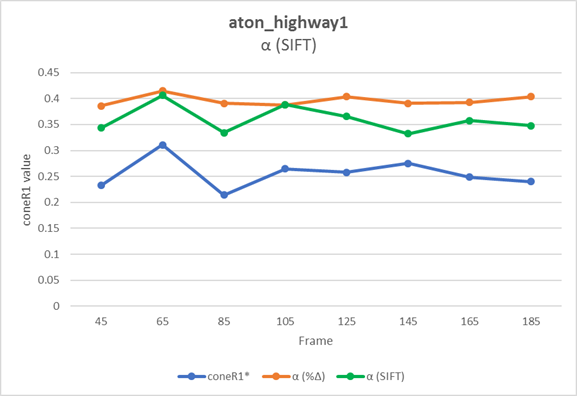
\includegraphics[width=1\linewidth]{figures/highway1_sift.jpg}
\caption{Low-contrast SIFT modulation's effect on correlation (y-axis) for aton\_highway1.}
\label{fig:highway1_sift}
\end{figure}

\begin{figure}
  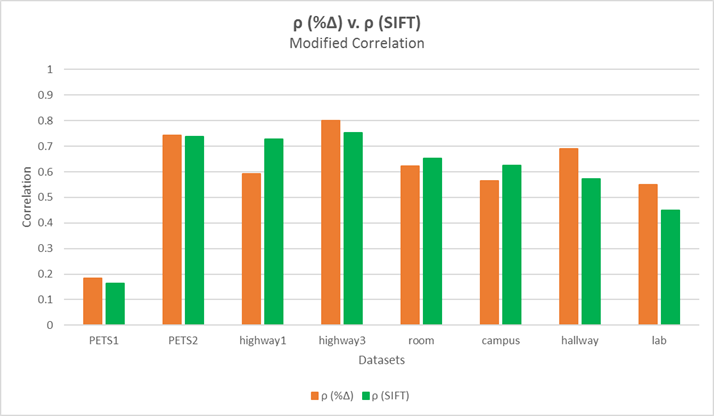
\includegraphics[width=1\linewidth]{figures/sift_correlation_diff.jpg}
\caption{Low-contrast SIFT modulation's effect on correlation (y-axis) for each dataset.}
\label{fig:corr_diff_sift}
\end{figure}

% Table Form (SIFT Diff)
\begin{table}
\centering
\begin{tabular}{ |c|c| }
	\hline
	\textbf{Dataset} & Correlation Diff (\%) \\
	\hline
	\hline
	\textbf{PETS1} &  -2.06 \\
	\hline
	\textbf{PETS2} & -0.58 \\
	\hline
	\textbf{aton\_highway1} &  13.62 \\
	\hline
	\textbf{aton\_highway3} & -4.76  \\
	\hline
	\textbf{aton\_room} & 3.087 \\
	\hline
	\textbf{aton\_campus} & 6.06 \\
	\hline
	\textbf{aton\_hallway} & -11.78 \\
	\hline
	\textbf{aton\_lab} & -10.17 \\
	\hline
\end{tabular}
\caption{Datasets and their correlations to \textit{coneR1} (\%$\Delta$ attenuation model).}
\label{table:corr_diff_sift}
\end{table}

While modulating the observed attenuation proved fruitful in some cases (aton\_highway1, aton\_room, aton\_campus), the negative affectation inflicted upon other datasets is too unpredictable and severe to warrant inclusion in the final generalized improvement model. Future work entails developing a more precise model to better abstract perceived quantities of shadows within a scene.

%%%
\section{Brightness Models and Correlation} \label{section:brightness_models}
%%%

In addition to differing responses to attenuation models, datasets also respond uniquely to varying brightness models. Figure \ref{fig:brightness_example} visualizes the disparity between multiple modes of brightness calculation, and how it may affect the correlation coefficient of attenuation. Tables \ref{table:brightness_corr_db} and \ref{table:brightness_corr_rgb} enumerate the correlative changes experienced by each dataset when subjected to multiple modes of brightness calculation.

% example 
\begin{figure}
\centering
\begin{subfigure}{.49\linewidth}
  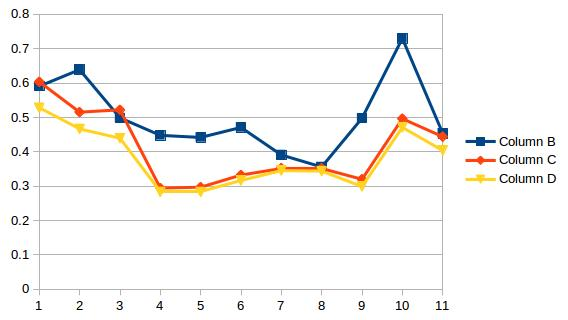
\includegraphics[width=1\linewidth]{figures/brightness/rgb/pets2_hsv_hsp.jpg}
  \caption{PETS2}
\end{subfigure}
\hfill
\begin{subfigure}{.49\linewidth}
  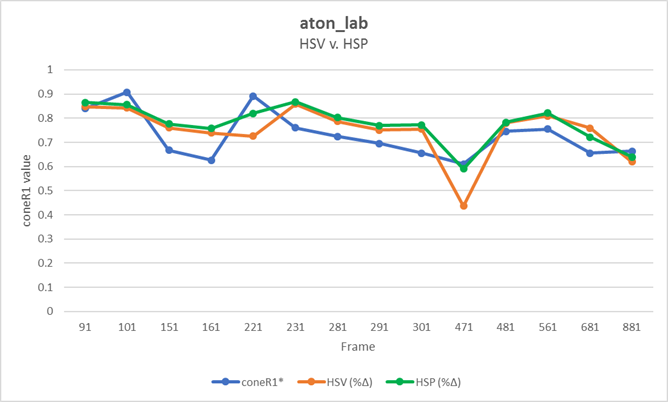
\includegraphics[width=1\linewidth]{figures/brightness/rgb/lab_hsv_hsp.jpg}
  \caption{aton\_lab}
\end{subfigure}

\caption{Example contrasting correlation improvements of the \%$\Delta$-HSP model (yellow) against \%$\Delta$-HSV (red) and optimal \textit{coneR1} (blue). }
\label{fig:brightness_example}
\end{figure}

% Table Form ((dB) Corr v. Brightness
\begin{sidewaystable}
\centering
\begin{tabular}{ |c|c|c|c|c|c|c|c| }
	\hline
	\textbf{Dataset} & \textbf{HSV} & \textbf{HSP} & \textbf{HSI} & \textbf{HSL}& \textbf{Y'} & \textbf{Norm} \\
	\hline
	\hline
	\textbf{PETS1} & 0.19855 & 0.22677 & 0.20217 & 0.18961 & 0.22215 & 0.20463 \\
	\hline
	\textbf{PETS2} & 0.67058 & 0.70576 & 0.68969 & 0.65327 & 0.69573 & 0.69453 \\
	\hline
	\textbf{aton\_highway1} & 0.68368 & 0.47716 & 0.52357 & 0.56044 & 0.47077 & 0.66944 \\
	\hline
	\textbf{aton\_highway3} & 0.74241 & 0.81413 & 0.79460 & 0.78019 & 0.81587 & 0.77326 \\
	\hline
	\textbf{aton\_room} & 0.54775 & 0.52845 & 0.53248 & 0.53619 & 0.52740 & 0.53179 \\
	\hline
	\textbf{aton\_campus} & 0.35996 & 0.48284 & 0.43049 & 0.41630 & 0.48696	 & 0.41998 \\
	\hline
	\textbf{aton\_hallway} & 0.65615 & 0.62531 & 0.61743 & 0.62235 & 0.61778 & 0.60148 \\
	\hline
	\textbf{aton\_lab} & 0.69540 & 0.70960 & 0.70478 & 0.71746 & 0.71005 & 0.70788 \\
	\hline
\end{tabular}
\caption{Datasets and their correlations to \textit{coneR1} (dB attenuation model) against Brightness models.}
\label{table:brightness_corr_db}
\end{sidewaystable}

% Brightness Models (dB)
%\begin{figure}
\begin{sidewaysfigure}
  \includegraphics[width=\linewidth]{figures/brightness/db/correlation_x.jpg}
  \caption{\textbf{REMOVE W3C!}}
\label{fig:brightness_corr_db}
%\end{figure}
\end{sidewaysfigure}

% Table Form (RGB) Corr v. Brightness
\begin{sidewaystable}
\centering
\begin{tabular}{ |c|c|c|c|c|c|c|c| }
	\hline
	\textbf{Dataset} & \textbf{HSV} & \textbf{HSP} & \textbf{HSI} & \textbf{HSL}& \textbf{Y'} & \textbf{Norm} \\
	\hline
	\hline
	\textbf{PETS1} & 0.18377 & 0.31951 & 0.24093 & 0.22212 & 0.23915 & 0.31368 \\
	\hline
	\textbf{PETS2} & 0.74308 & 0.74107 & 0.74571 & 0.71711 & 0.74772 & 0.73219 \\
	\hline
	\textbf{aton\_highway1} & 0.59231 & 0.18923 & 0.39381 & 0.39631 & 0.31300 & 0.21639 \\
	\hline
	\textbf{aton\_highway3} & 0.80138 & 0.76171 & 0.80438 & 0.78177 & 0.81546 & 0.76015 \\
	\hline
	\textbf{aton\_room} & 0.62269 & 0.61823 & 0.62131 & 0.62163 & 0.62328 & 0.61681 \\
	\hline
	\textbf{aton\_campus} & 0.56459 & 0.37156 & 0.40715 & 0.39544 & 0.45946 & 0.36119 \\
	\hline
	\textbf{aton\_hallway} & 0.68973 & 0.42918 & 0.74614 & 0.75390 & 0.75638 & 0.40423 \\
	\hline
	\textbf{aton\_lab} & 0.55087 & 0.72925 & 0.59196 & 0.60837 & 0.59782 & 0.72522 \\
	\hline
\end{tabular}
\caption{Datasets and their correlations to \textit{coneR1} (\%$\Delta$ attenuation model) against Brightness models.}
\label{table:brightness_corr_rgb}
\end{sidewaystable}

% Brightness Models (RGB)
\begin{sidewaysfigure}
  \includegraphics[width=\linewidth]{figures/brightness/rgb/correlation_x.jpg}
  \caption{\textbf{REMOVE W3C!}}
\label{fig:brightness_corr_rgb}
\end{sidewaysfigure}

Two distinct response trends are observed in Figure \ref{fig:brightness_corr_db}. These trends are clearly shown in Figure \ref{fig:brightness_indoor_outdoor}: outdoor datasets (PETS1, PETS2, highway3, and campus) share a similar response to changing brightness models, while indoor datasets (room, hallway, and lab) also share a similar response. The difference in brightness models can be primarily characterized by their individual treatments of color content in a pixel. The grouping of datasets further reinforces the importance of color shift depending on the environment. We differentiate between the datasets by measuring red-green color bias present within cast shadows, defined as the observed blue color shift subtracted from the mean of observed red and green color shifts. As seen in Table \ref{make a table for this}, each outdoor dataset exhibits a red-green color bias of at least 2 units, while indoor datasets exhibit a red-green bias of less than 2 units.

It is important to note that Figure \ref{fig:brightness_corr_rgb} does not exhibit the trends indicated by the dB model in Figure \ref{fig:brightness_corr_db}. This is inherent to the model of attenuation itself. The \%$\Delta$ model of attenuation divides the vector from bg $\rightarrow$ fg by the RGB vector $\vec{bg}$ describing the illuminated background pixel. In this way, brightness change is calculated using the vector $\vec{bg \rightarrow fg}$. Some datasets, such as PETS1, PETS2, aton\_highway3, and aton\_room, demonstrate similar responses to those observed in Figure \ref{fig:brightness_corr_db}. However, aton\_lab, aton\_hallway, and aton\_campus behave erratically in comparison to their corresponding dB responses. The disparity between the two brightness responses can be attributed to color information captured by the \%$\Delta$ model that is discarded in the dB model.

The exception to this grouping of outdoor and indoor datasets is aton\_highway1, an outdoor dastaset that has a response reciprocal to that of most outdoor environments. Figure \ref{fig:highway1_reciprocal} visualizes the mirrored nature of aton\_highway1's response. In Chapter (methodology) in section (rgb shift), we can see aton\_highway1's RGB shift in shadowed regions (Figure \ref{}). The RGB shift is characteristic of an outdoor scene; red, green, and blue channels attenuate by different amounts. However, aton\_highway1 contains the darkest cast shadows in relation to its background model. The highest of aton\_highway1's responses, HSV and Norm, both result in an over-valued brightness value in accordance to color shifts. Norm is overvalued due to the Euclidean distance resultant lying outside the range \textit{min}(channel value) $<$ dist. $<$ \textit{max}(channel value), while HSV is overvalued due to its reliance on one channel. While HSV and Norm serve as relative low points in other outdoor datasets for that reason, the larger calculated brightness attenuation simply provided for a closer relational value with the optimal \textit{coneR1} value in the dark shadowed region.

% Brightness Models indoor/outdoor (dB)
\begin{figure}
\centering
\begin{subfigure}{.8\linewidth}
  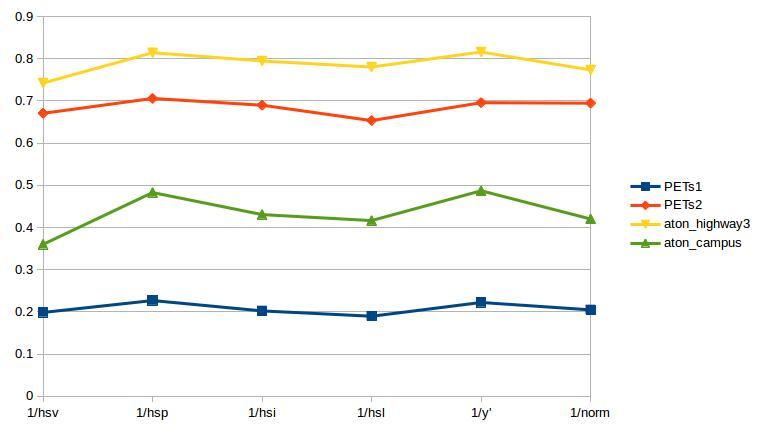
\includegraphics[width=1\linewidth]{figures/brightness/db/correlation_outside.jpg}
  \caption{}
\end{subfigure}
\hfill
\begin{subfigure}{.8\linewidth}
  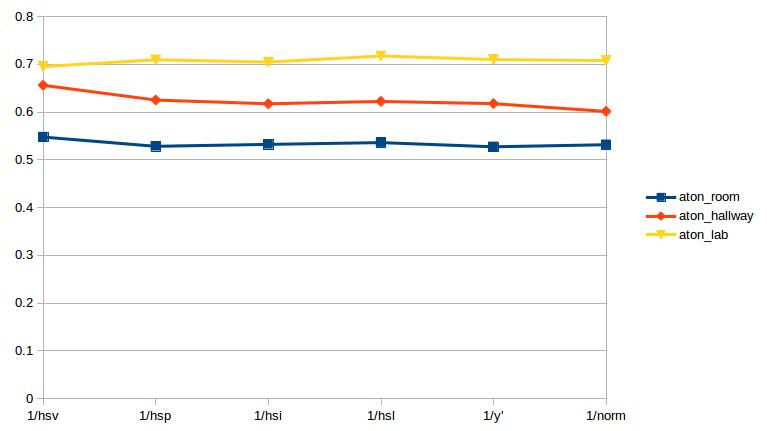
\includegraphics[width=1\linewidth]{figures/brightness/db/correlation_inside.jpg}
  \caption{}
\end{subfigure}

\caption{Outdoor datasets (a) share a common response to varying brightness models. In contrast, indoor datasets (b) share a common lack of response.}
\label{fig:brightness_indoor_outdoor}
\end{figure}

% Aton_highway1 oddity
\begin{figure}
\centering
  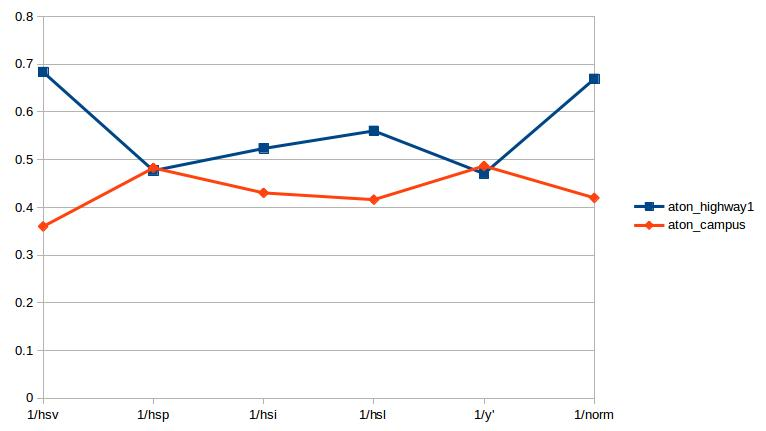
\includegraphics[width=1\linewidth]{figures/brightness/db/highway1_reciprocal.jpg}
\caption{aton\_highway1's response to various brightness models is foil to other outdoor datasets' responses.}
\label{fig:highway1_reciprocal}
\end{figure}

%%%
\section{Parameter Model Results}
%%%

The primary challenge in adapting observed average attenuation into an arbitrary model for shadow removal improvement lies in understanding the necessary translation between observed attenuation and optimally tuned \textit{coneR1}. Utilizing the formula specified in Chapter (methodology) in section (param model), a coarse-grained model was developed. Applied to an arbitrary frame, attenuation and color magnitude shift is analyzed and used to create the necessary translation. This analysis is performed on each brightness model, seen in Figure \ref{fig:model_scatter}. For each brightness model, red-green color bias in shadow pixels is plotted against the RSO (Required Shift to Optimal) between optimally \textit{coneR1} and observed attenuation. A best-fit logarithm is drawn for each of these scatterplots, relating required attenuation translation and observed color-bias. Visualized results of this combination model are displayed in Figure \ref{fig:new_coneR1}. The resultant of the model, shown in \textbf{red (this might change)}, retains correlative properties observed prior while providing a reasonable estimate for required translation.

% RGB shift per req. shift to optimal
\begin{figure}
\centering
\begin{subfigure}{.49\linewidth}
  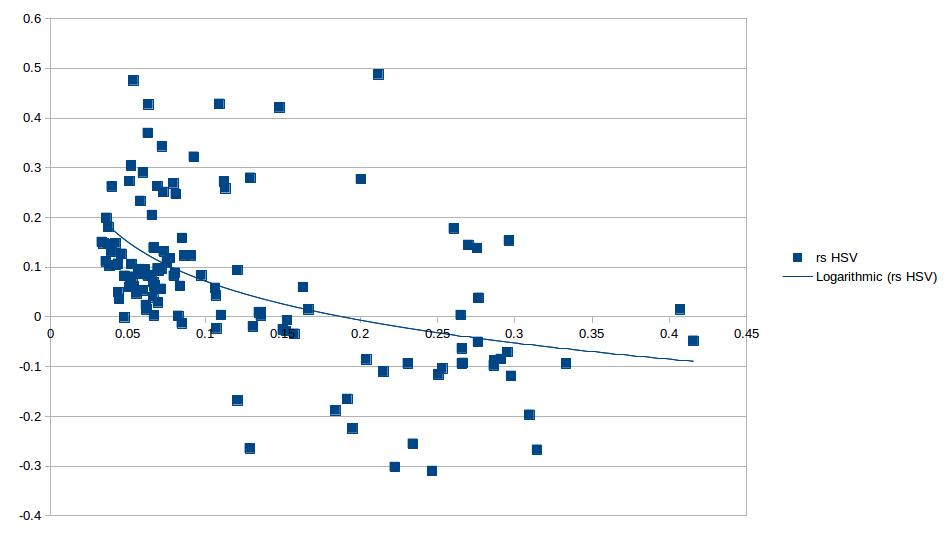
\includegraphics[width=1\linewidth]{figures/model/scatter/model_hsv.jpg}
  \caption{HSV}
\end{subfigure}
\hfill
\begin{subfigure}{.49\linewidth}
  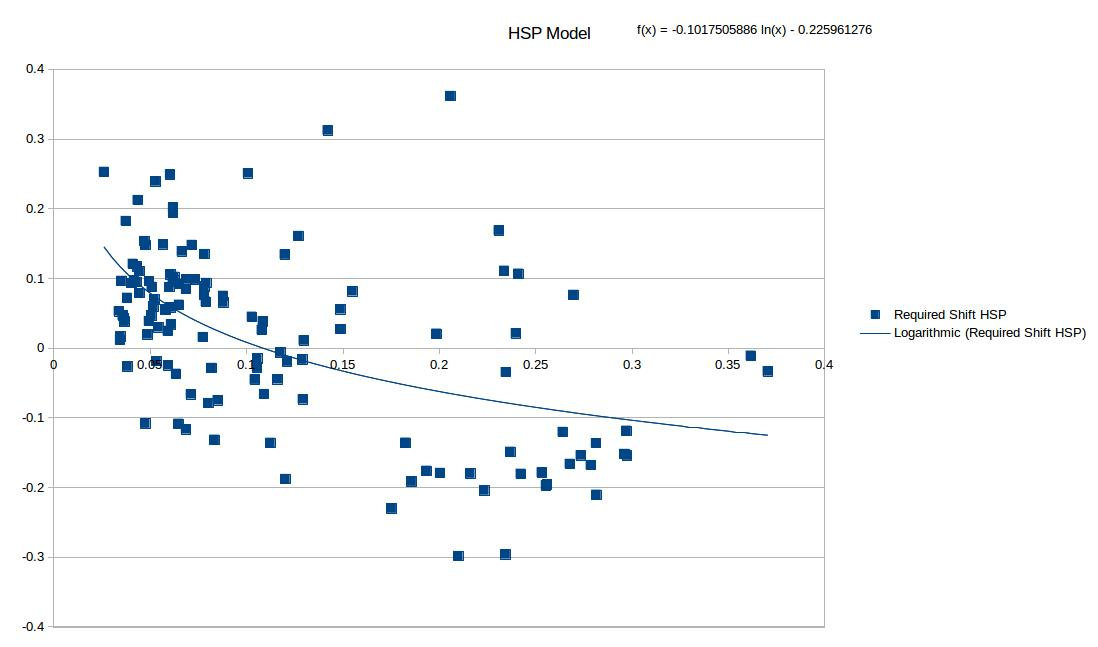
\includegraphics[width=1\linewidth]{figures/model/scatter/model_hsp.jpg}
  \caption{HSP}
\end{subfigure}
\hfill
\begin{subfigure}{.49\linewidth}
  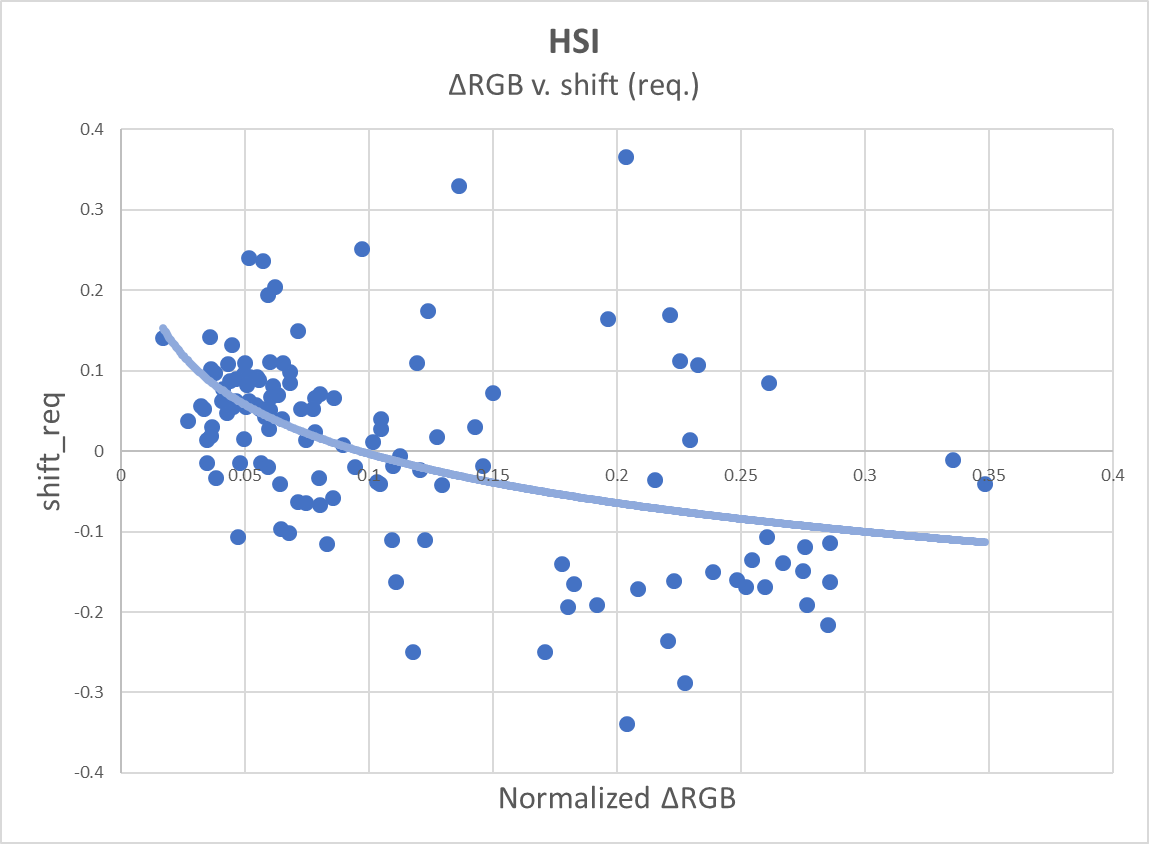
\includegraphics[width=1\linewidth]{figures/model/scatter/model_hsi.jpg}
  \caption{HSI}
\end{subfigure}
\hfill
\begin{subfigure}{.49\linewidth}
  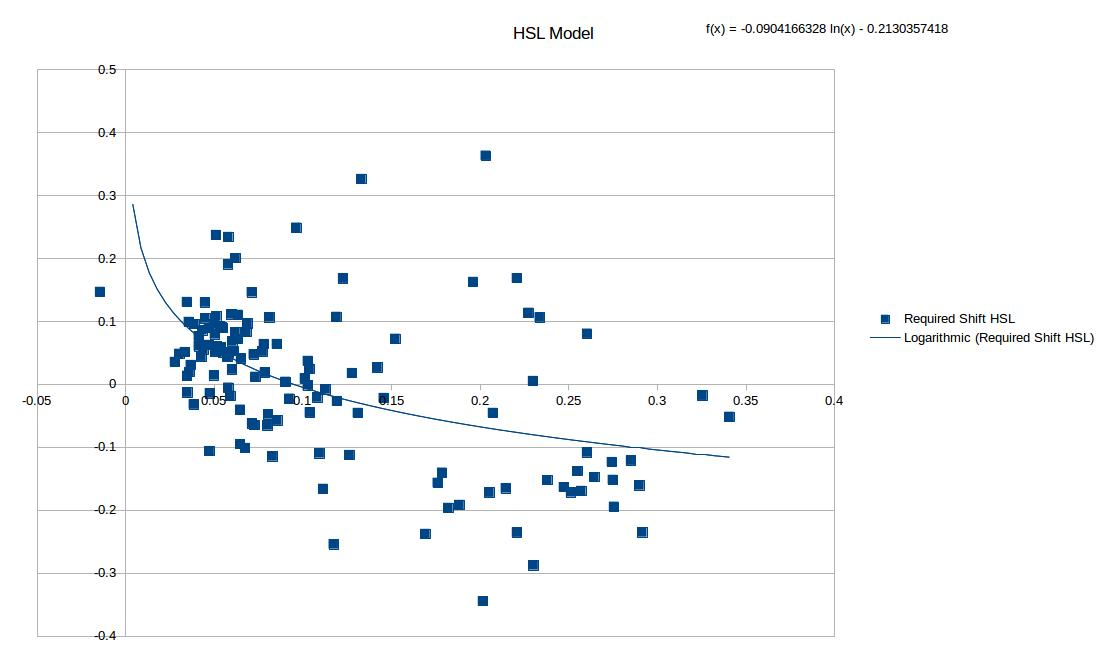
\includegraphics[width=1\linewidth]{figures/model/scatter/model_hsl.jpg}
  \caption{HSL}
\end{subfigure}
\hfill
\begin{subfigure}{.49\linewidth}
  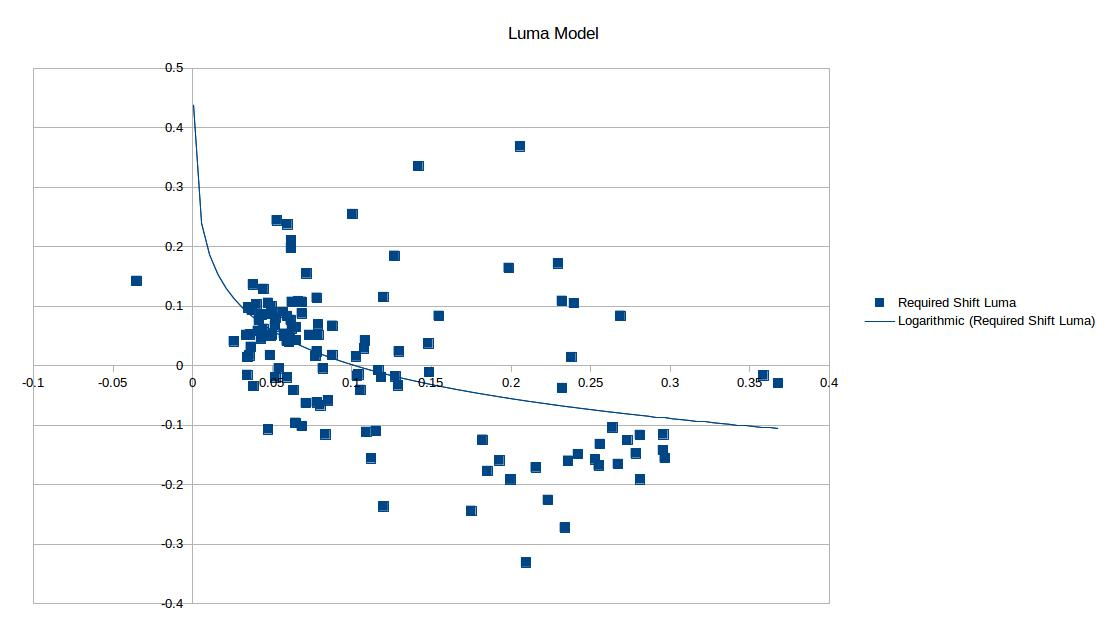
\includegraphics[width=1\linewidth]{figures/model/scatter/model_luma.jpg}
  \caption{Luma (Y')}
\end{subfigure}
\hfill
\begin{subfigure}{.49\linewidth}
  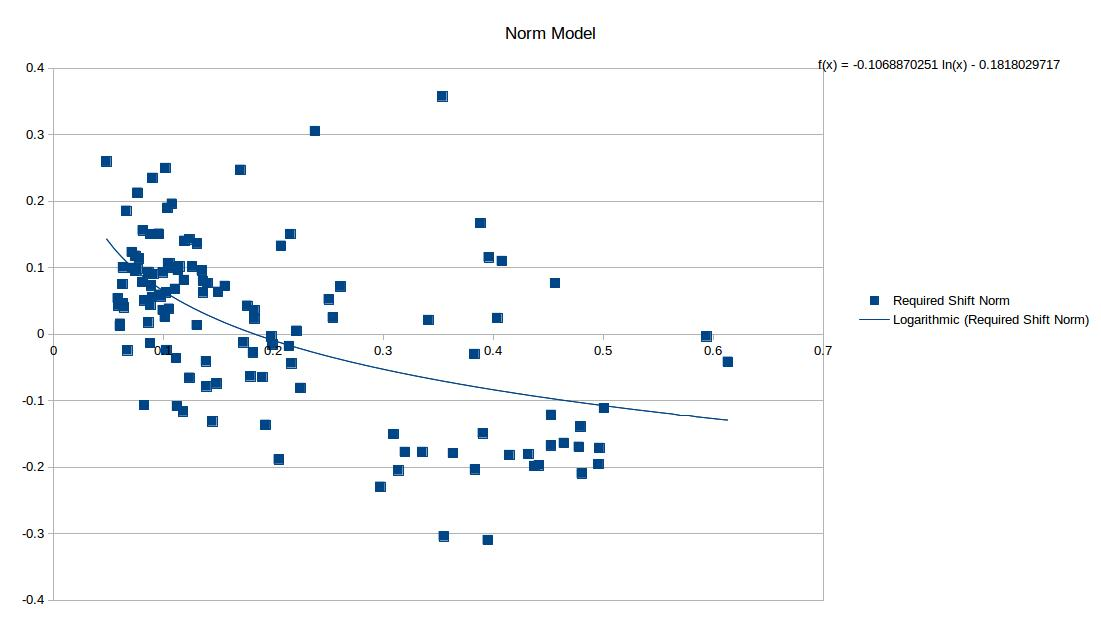
\includegraphics[width=1\linewidth]{figures/model/scatter/model_norm.jpg}
  \caption{Norm}
\end{subfigure}

\caption{For each brightness model, red-green color bias is plotted against RSO \textbf{define this in methodology}. The general model for each brightness calculation is formed through a best-fit logarithm.}
\label{fig:model_scatter}
\end{figure}

% coneR1 v. newR1
\begin{figure}
  \centering
  \begin{subfigure}{1\linewidth}
  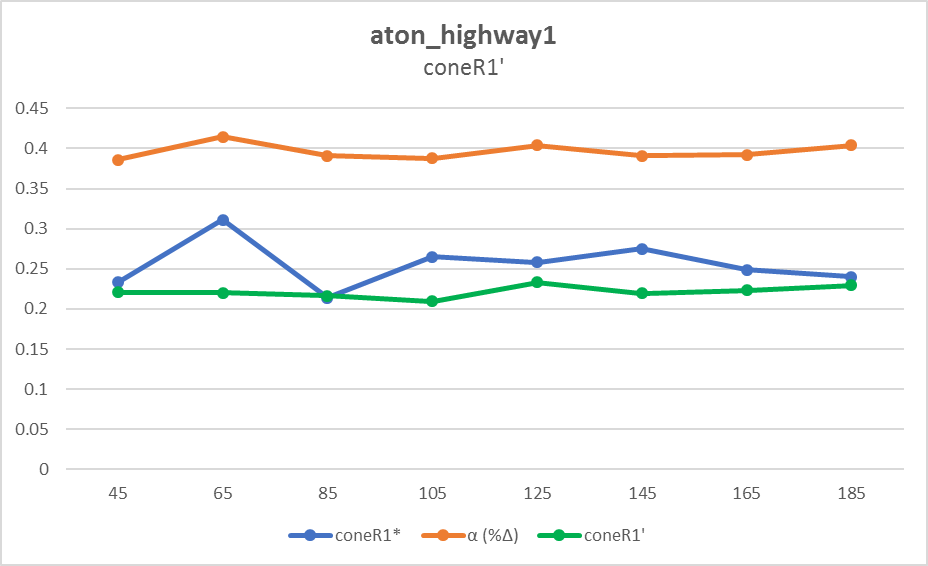
\includegraphics[width=1\linewidth]{figures/model/highway1_calc_coneR1.jpg}
  \caption{}
\end{subfigure}
\hfill
\begin{subfigure}{1\linewidth}
  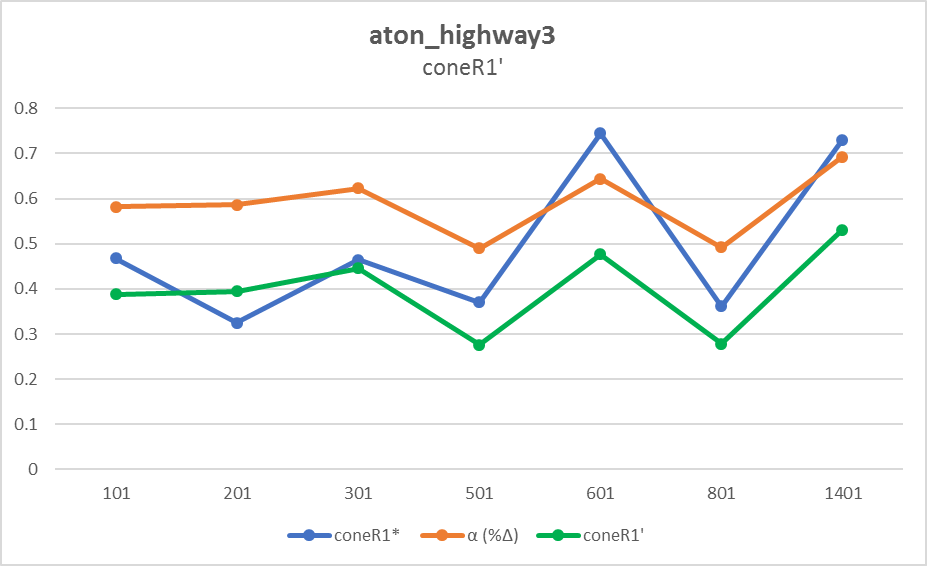
\includegraphics[width=1\linewidth]{figures/model/highway3_calc_coneR1.jpg}
  \caption{}
\end{subfigure}

\caption{Automatically tuned \textit{coneR1} parameter (orange) charted against optimally tuned \textit{coneR1} parameter (blue) and average attenuation (\%$\Delta$) (yellow). All results can be found in the appendix.}
\label{fig:new_coneR1}
\end{figure}

\subsection{Analysis}

Figure \ref{fig:bars_hsv_calc} provides the resulting detection and discrimination rates of shadow removal using the programmatically-generated parameter, contrasting the generated results (orange) with detection/discrimination determined via the original naive method (blue). Quantitative results are shown in Table \ref{plstablenow}. Results indicate that for a majority of datasets, fractional amount of shadow detection are sacrificed for disproportionate increases in discrimination of shadows. \textbf{Figure \ref{qualgraphic}} qualitatively visualizes shadow removal improvements using the adaptive method.

% detect/discrim calc
\begin{figure}
\centering
\begin{subfigure}{1\linewidth}
  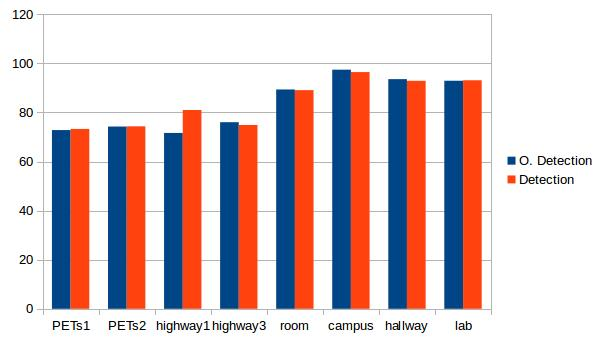
\includegraphics[width=1\linewidth]{figures/model/detect_hsv.jpg}
  \caption{}
\end{subfigure}
\hfill
\begin{subfigure}{1\linewidth}
  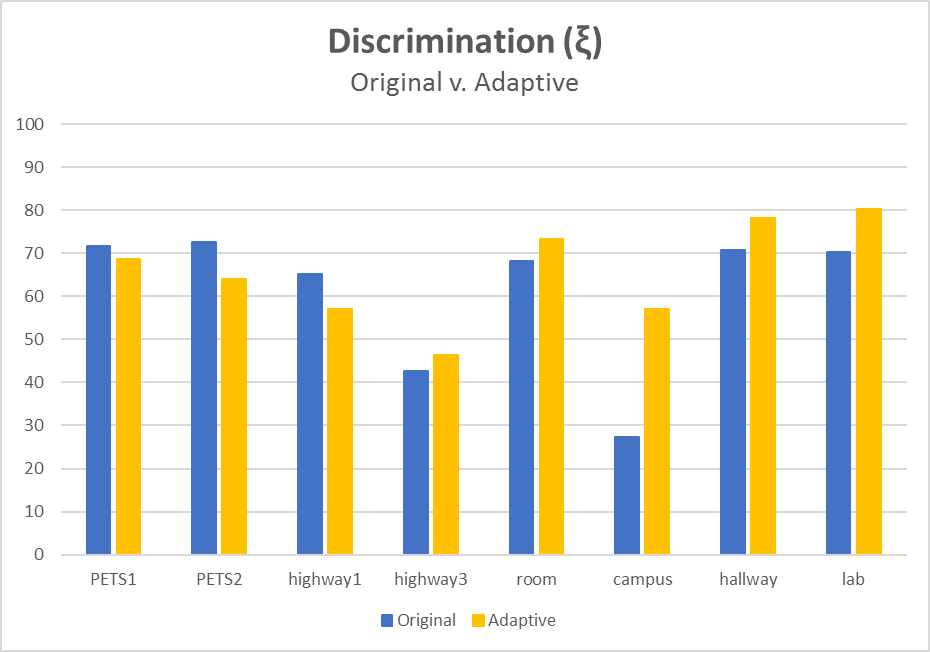
\includegraphics[width=1\linewidth]{figures/model/discrim_hsv.jpg}
  \caption{}
\end{subfigure}

\caption{Detection (a) and Discrimination (b) calculated using the HSV parameter model, for each dataset.}
\label{fig:bars_hsv_calc}
\end{figure}

\begin{figure}
  \centering
  \begin{subfigure}{.49\linewidth}
  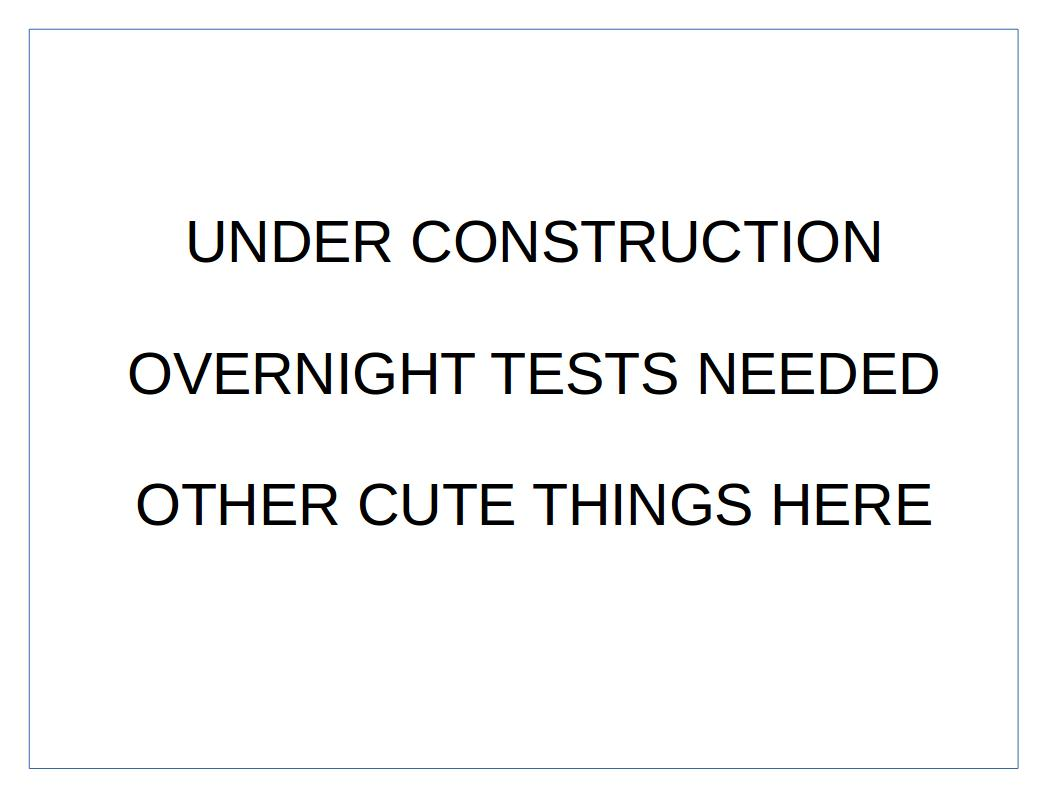
\includegraphics[width=1\linewidth]{figures/placeholder.jpg}
  \caption{}
  \end{subfigure}
  \hfill
  \begin{subfigure}{.49\linewidth}
  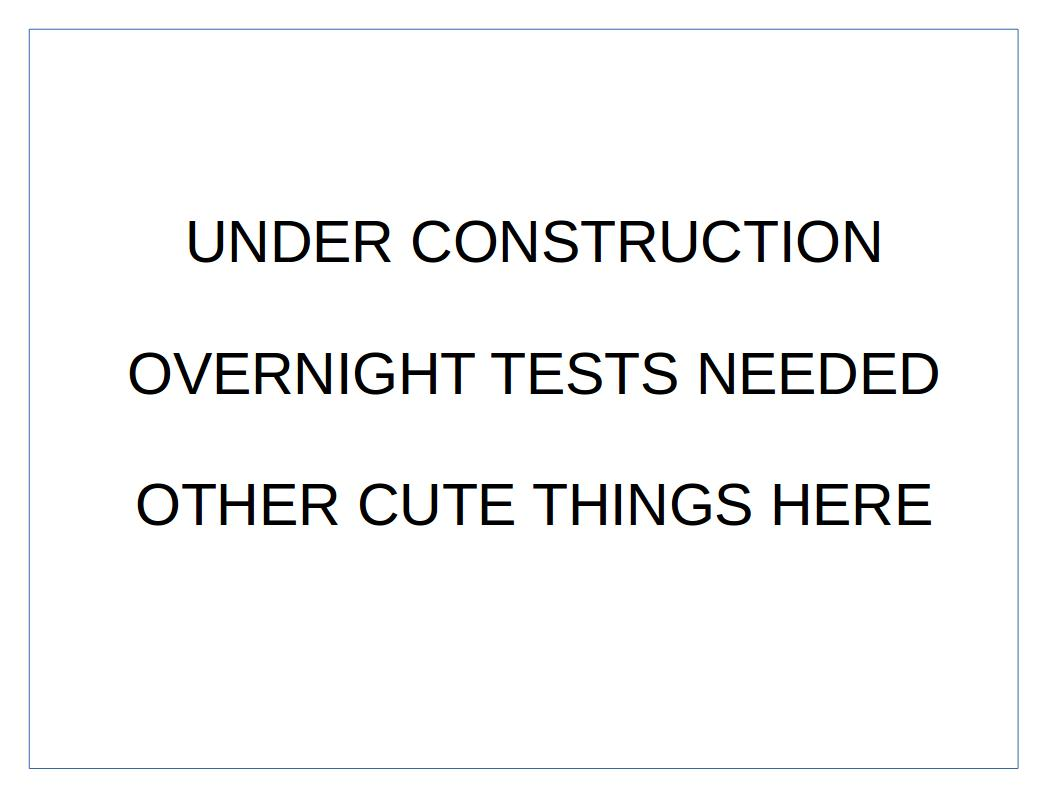
\includegraphics[width=1\linewidth]{figures/placeholder.jpg}
  \caption{}
  \end{subfigure}
  \hfill
  \begin{subfigure}{.49\linewidth}
  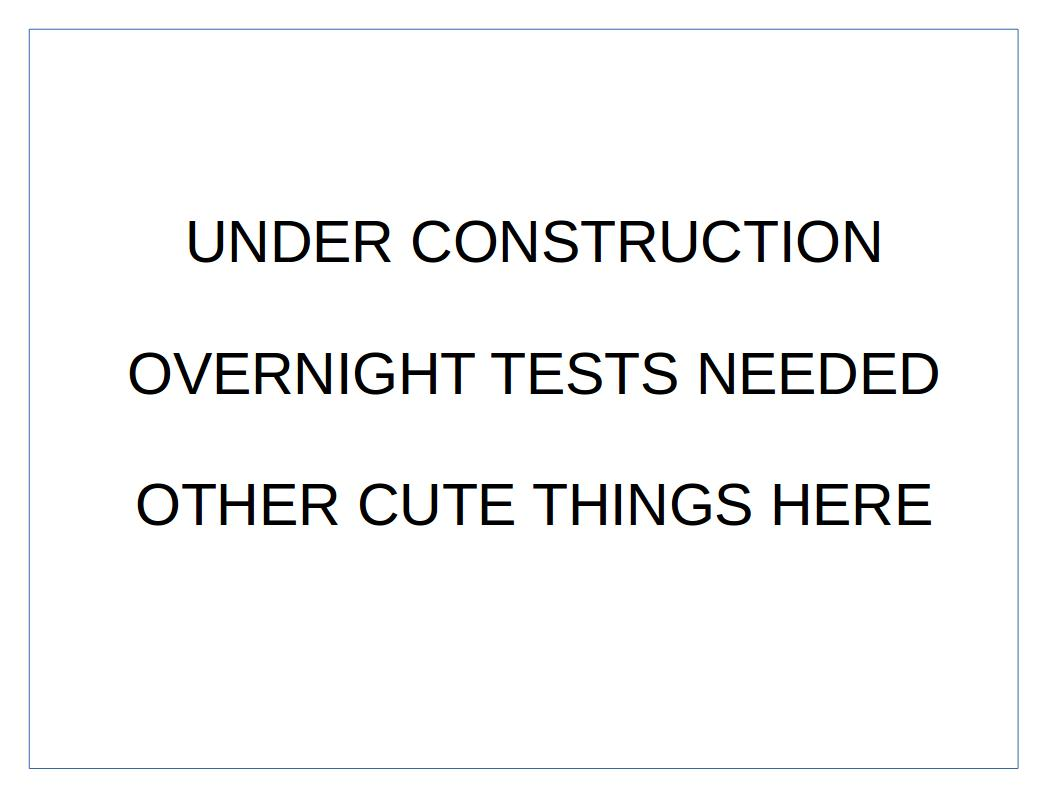
\includegraphics[width=1\linewidth]{figures/placeholder.jpg}
  \caption{}
  \end{subfigure}
  \hfill
  \begin{subfigure}{.49\linewidth}
  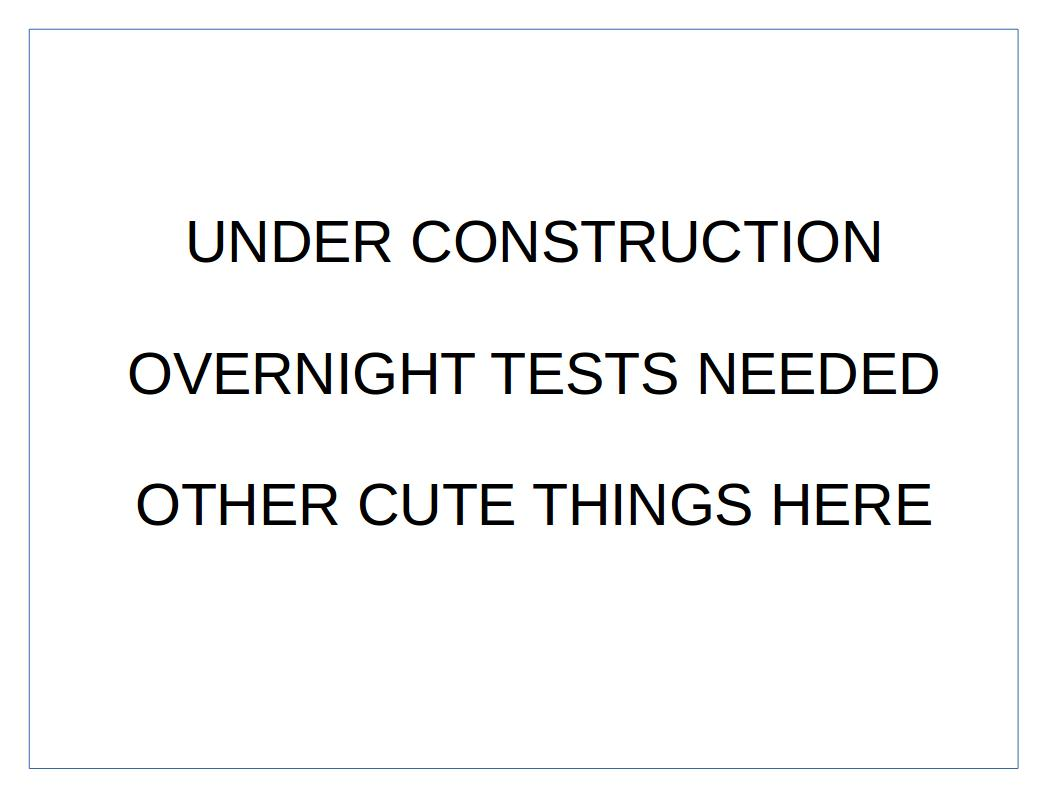
\includegraphics[width=1\linewidth]{figures/placeholder.jpg}
  \caption{}
  \end{subfigure}
\caption{Qualitative shadow removal improvement.}
\label{fig:qual_results}
\end{figure} 

aton\_highway1 proved consistently anomalous \textbf{woo oxymorons}, trading in nearly equal part detection for discrimination, arriving at a net modest positive of 1.2\%. We theorize aton\_highway1's unwaveringly inconsistent \textbf{I enjoy oxymorons, okay} behavior is again due to it possessing the darkest cast shadows. Furthermore, as seen in Figure \ref{color bias ref}, aton\_highway1 attenuates non-linearly (as expected of an outdoor scene), yet by visual inspection, is desaturated to the point of grayscale. The combination of the strong shadows, the low saturation of the frame, and the relative featureless nature of the background model, allows a larger population of candidate shadows pixels to be gathered. Due to these conditions, foreground \textit{object} pixels are more likely to appear identical to shadow pixels, in both color information and relative distance from its background pixel. The confluence of these scene characteristics renders aton\_highway1 less predictable than other datasets.

PETS1 and PETS2 also do not conform to the upward trends seen in the majority of datasets. In the case of PETS1, the root cause is hypothesized to be similar to the reason for the low correlation coefficient, i.e., a non-ideal background model that misrepresents the attenuation of cast shadows. More interestingly, PETS2 experiences the same degradation of performance as PETS1, but has a much stronger correlation coefficient, seen in Table \ref{table:corr_rgb}. This decoupling of correlation and accuracy stems from the generalized model of improvement translating the observed average attenuation necessarily. This is visualized in Figure \ref{fig:pets2_translate}. The model overcompensates for observed color bias in PETS2, and again the culprit is the non-ideal background model. The misrepresentation of attenuation (and thereby color bias) of cast shadows in PETS2 results in the unnecessary 'downward' translation, impacting PETS2's shadow discrimination accuracy.

\begin{figure}
  \centering
  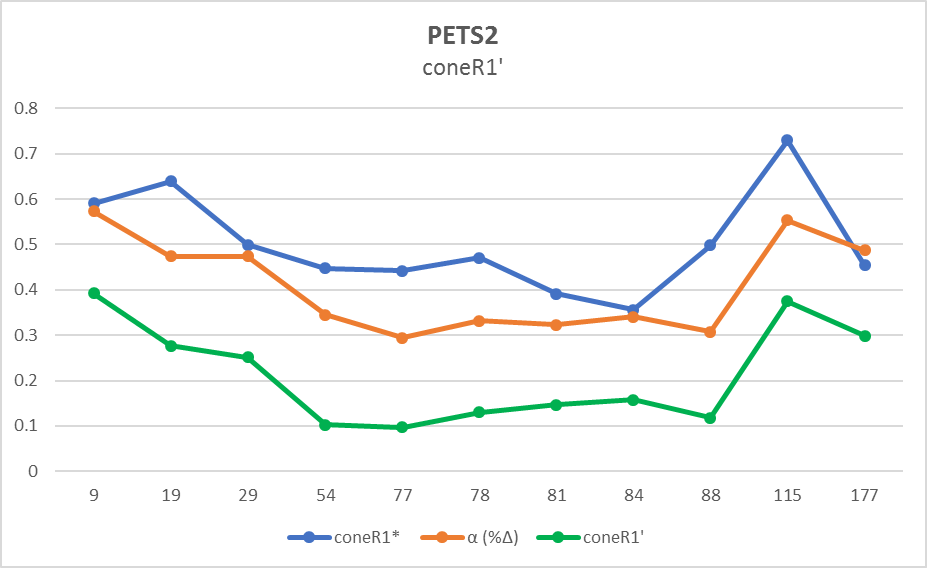
\includegraphics[width=1\linewidth]{figures/model/pets2_translate.jpg}
\caption{}
\label{fig:pets2_translate}
\end{figure} 

\subsection{Brightness Models and Shadow Removal}

It is noted in section \ref{section:brightness_models} that the correlative changes observed in varying brightness models are not consistent from the dB to the \%$\Delta$ model of attenuation. While correlation coefficient and shadow removal improvement are often related, it is entirely possible to observe cases in which the opposite is true. For example, two vectors are perfectly correlated, $a^T$ = [20, 10] and $b^T$ = [10, 0]. By increasing $b^T$ to [10, 10], the vectors' correlation coefficient is greatly reduced, while their overall fit has been improved. The following results demonstrate this concept, uncoupling the correlation changes recorded in section \ref{section:brightness_models} from shadow removal improvement. Figure \ref{fig:pets1_bars_calc_all} illustrates detection (blue) and discrimination (orange) rates within a dataset across varying brightness modes.

% HSV, HSP, etc for one dataset
\begin{figure}
\centering
  \begin{subfigure}{1\linewidth}
  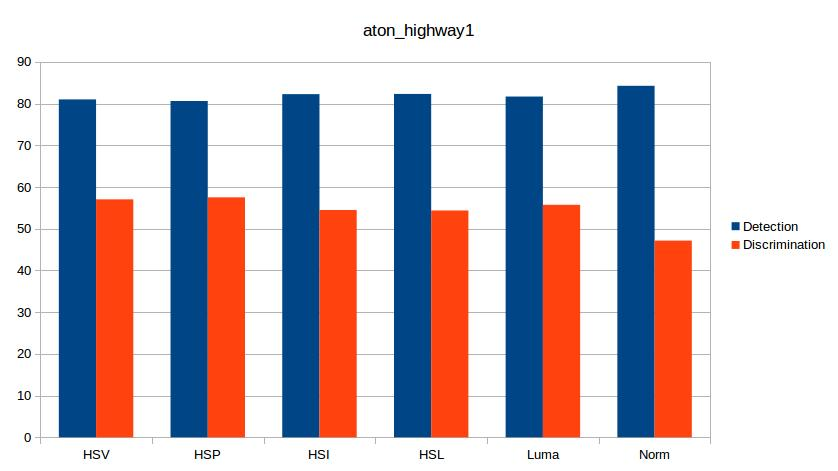
\includegraphics[width=1\linewidth]{figures/model/highway1_all_brightness_models.jpg}
  \caption{aton\_highway1}
\end{subfigure}
\hfill
  \begin{subfigure}{1\linewidth}
  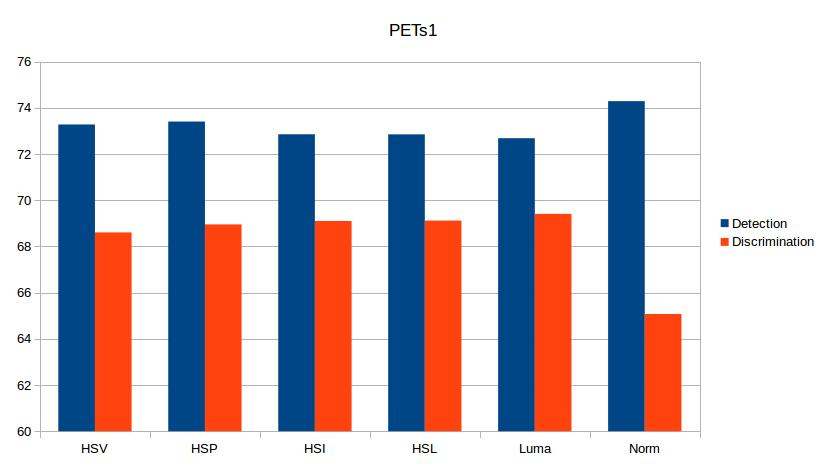
\includegraphics[width=1\linewidth]{figures/model/pets1_all_brightness_models.jpg}
  \caption{PETS1}
\end{subfigure}
\caption{Detection (blue) and Discrimination (orange) for each brightness model. Full results for all datasets can be found in the appendix.}
\label{fig:pets1_bars_calc_all}
\end{figure}

The effect of varying brightness models on shadow removal improvement loosely adheres to trends identified in section \ref{section:brightness_models}. Marginal improvements are found using the HSP brightness model for most outdoor scenes, while the default HSV brightness model performed better for indoor scenes. While the improvements are marginal, the results on display validate the claim that brightness models that incorporate color information provide better shadow removal for outdoor scenes, while brightness models that analyze only intensity improve shadow removal for indoor scenes.

\end{document}
